\chapter{Дифференциалы и производные}

\section{Определение}
Производная -- предел отношения приращения функции к приращению её аргумента при стремлении 
приращения аргумента к нулю, если такой предел существует.\newline
$\displaystyle f(x)^{'} =\lim_{\Delta x \to 0} \frac{f(x + \Delta x) - f(x)}{\Delta x}$\newline

Диффенциал -- произведение производной на приращение аргумента. Дифференциал функции $f$ в точке $a$ 
обозначается $df_a$.\newline\newline
Пусть $f: {<}{a,\ b}{>} \rightarrow \mathbb{R}$ и $x_0 \in {<}{a,\ b}{>}$. Тогда функция $f$ 
дифференцируема в точке $x_0$, если $\exists A \in \mathbb{R}:\ f(x) - f(x_0) = A(x-x_0) + o(x - 
x_0)$.\newline
Обозначим за $h$ приращение аргумента: $h = x - x_0$.
Тогда дифференциал этой функции может быть записан так:\newline
$d_{x_0}f(h) = A \cdot h$\newline
А приращение функции так:\newline\newline
$f(x_0 + h) - f(x_0) = \underbrace{\overbrace{A}^{\mathclap{\text{производная}}} \cdot 
h}_{\mathclap{\text{глав. линейная часть приращ. функции}}} + o(h)$\newline

\section{Производные некоторых функций}
\begin{enumerate}
\item $(c)^{'}=0$
\item $(x^n)^{'} = nx^{n-1}$
\item $(n^x)^{'} = n^x \ln{n}$
\item $(\log_n(x))^{'} = \frac{1}{x \ln {n}}$
\item $\cos{x}^{'} = -\sin{x}$
\item $\sin{x}^{'} = \cos{x}$
\item $\tg{x}^{'} = \frac{1}{\cos^2{x}}$
\item $\ctg{x}^{'} = \frac{1}{-\sin^2{x}}$
\item $\arcsin{x}^{'} = \frac{1}{\sqrt{1-x^2}}$
\item $\arccos{x}^{'} = -\frac{1}{\sqrt{1-x^2}}$
\item $\arctg{x}^{'} = \frac{1}{1+x^2}$
\item $\arcctg{x}^{'} = -\frac{1}{1+x^2}$
\item $(e^x)^{'} = e^x$
\end{enumerate}

\section{Критерий дифференциируемости}
\begin{theorem}
Следующие условия равносильны:
\begin{enumerate}
\item f -- дифференцируема в точке $x_0$  и её производная -- $A$
\item $\displaystyle \exists \lim_{h \to 0} \frac{f(x_0 + h) - f(x_0)}{h} \in \mathbb{R} = A$
\item $\exists f(x)$ -- непрерывная в точке $x_0:\ f(x) = f(x_0) + F(x)(x - x_0)$
\end{enumerate}
\end{theorem}
\circled{1} $\Longrightarrow$ \circled{2}\newline
Т.к. $f$ -- дифференциируема в т. $x_0$:\newline
$f(x) = f(x_0) + A(x - x_0) + o(x - x_0)$ (при $x \to x_0$)\newline
$\displaystyle \lim_{h \to 0} \frac{f(x_0 + h) - f(x_0)}{h} = \lim_{h\to 0} \frac{A\cdot h + 
o(h)}{h} = A$\newline\newline

\circled{2} $\Longrightarrow$ \circled{3}\newline



\section{Правило Лопиталя}
\subsection{Раскрытие неопределенноти вида $\frac{0}{0}$}
\begin{theorem}$ \exists a, b : \begin{cases} a < b \\ f, g - $ дифференцируемы на $ (a, b), \\ 
\displaystyle \lim_{ x \to a+}f(x) = \lim_{x \to a+}g(x) = 0, \\ \forall x \in (a, b) : g^{'}(x) 
\neq 0, \\ \displaystyle \exists \lim_{x \to a+}\frac{f^{'}(x)}{g^{'}(x)} = L \in \overline{R}; 
\end{cases}$ $\Longrightarrow$ $\displaystyle \lim_{x \to a+}\frac{f(x)}{g(x)} = L$ \end{theorem}
Для доказательства рассмотрим два случая. \\
1) $a \in R$\\
\begin{center}
  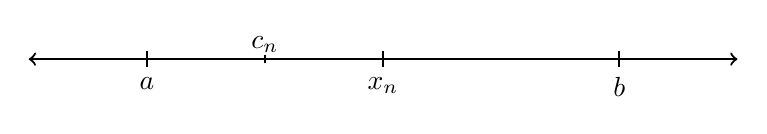
\begin{tikzpicture}[thick]
    \draw[thick, <->](0.5,0)--(9.5,0);
    \foreach \x/\xtext in {2/$a$, 5/$x_n$, 8/$b$}
      \draw(\x,3pt)--(\x,-3pt) node[below] {\xtext};
    \foreach \x/\xtext in {3.5/$c_n$}
      \draw(\x, 1.5pt)--(\x,-1.5pt) node[above] {\xtext};
  \end{tikzpicture}
 \end{center}
Определим последовательность $x_n$ следующим образом $ x_n \underset{n \to \infty}{\to} a+$ \\ 
Другими словами: $x_n \in (a, b), x_n \underset{n \to \infty}{\to} a$ \\ 
Доопределим (или переопределим) $f$ и $g$ : \\
$f(a) = g(a) = 0$\\
$f, g$ - дифференцируемы на $(a, x_n)$ и непрерывны на $[a, x_n]$. Значит по теореме Коши $\exists 
c_n \in (a, x_n):$\\\\
$\displaystyle 
\frac{f(x_n)-f(a)^{\rotatebox{40}{\text{=0}}}}{g(x_n)-g(a)_{{\rotatebox{-40}{\text{=0}}}}} = 
\frac{f^{'}(c_n)}{g^{'}(c_n)} = \frac{f(x_n)}{g(x_n)}$


